% Created 2023-02-22 Wed 19:49
% Intended LaTeX compiler: pdflatex
\documentclass[11pt]{article}
\usepackage[utf8]{inputenc}
\usepackage[T1]{fontenc}
\usepackage{graphicx}
\usepackage{longtable}
\usepackage{wrapfig}
\usepackage{rotating}
\usepackage[normalem]{ulem}
\usepackage{amsmath}
\usepackage{amssymb}
\usepackage{capt-of}
\usepackage{hyperref}
\author{Diego Domínguez}
\date{\today}
\title{Direccionamiento IP}
\hypersetup{
 pdfauthor={Diego Domínguez},
 pdftitle={Direccionamiento IP},
 pdfkeywords={},
 pdfsubject={},
 pdfcreator={Emacs 28.2 (Org mode 9.6)}, 
 pdflang={English}}
\begin{document}

\maketitle
\tableofcontents

\begin{itemize}
\item Juntar las dos subredes
\item 

\item Establecer
\begin{itemize}
\item Máscaras
\item Red
\item Broadcast
\item Rango útil
\item Red
\end{itemize}
\end{itemize}


\begin{center}
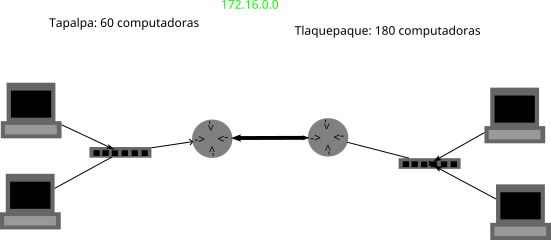
\includegraphics[width=.9\linewidth]{./ejercicio.png}
\end{center}


\section{Tlaquepaque}
\label{sec:org76f7239}
\begin{itemize}
\item Network: 172.16.0.0
\item Mask: 255.255.255.0
\item Broadcast: 172.16.0.255
\item Rango útil: 172.16.0.1 -> 172.16.0.254
\item Gateway: 172.16.0.254
\end{itemize}

\section{Tapalpa}
\label{sec:org0fdda6a}
\begin{itemize}
\item Network: 172.16.1.0
\item Mask: 255.255.255.192
\item Broadcast: 172.16.1.63
\item Rango útil: 172.16.1.1 -> 172.16.1.62
\item Gateway: 172.16.1.62
\end{itemize}

\section{Enlace Tapalpa - Tlaquepaque}
\label{sec:org09a9927}
\begin{itemize}
\item Network: 172.16.1.64
\item Mask: 255.255.255.252
\item Broadcast: 172.16.1.67
\item Rango útil: 172.16.1.65 -> 172.16.1.66
\end{itemize}




\begin{center}
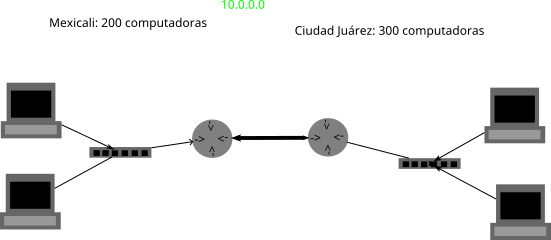
\includegraphics[width=.9\linewidth]{./ejercicio2.png}
\end{center}
\end{document}